\documentclass[12pt]{article}

\usepackage{amsmath}
\usepackage{amssymb}
\usepackage{anyfontsize}
\usepackage[toc,page]{appendix}
\usepackage{array}
\usepackage{booktabs}
\usepackage{caption}
\usepackage{cellspace}
\usepackage{color}
\usepackage{enumerate}
\usepackage{enumitem}
\usepackage{float}
\usepackage{geometry}
\usepackage{graphicx}
\usepackage{newtxtext,newtxmath}
\usepackage{listings}
\usepackage{physics} 
\usepackage{subfigure}
\usepackage{tabularx}

\geometry{
    a4paper,
    total = {170mm, 257mm},
    left = 20mm,
    top = 20mm,
    }

\definecolor{dkgreen}{rgb}{0,0.6,0}
\definecolor{gray}{rgb}{0.5,0.5,0.5}
\definecolor{mauve}{rgb}{0.58,0,0.82}
\lstset{frame = tb,
        language = Python,
        aboveskip = 3mm,
        belowskip = 3mm,
        showstringspaces = False,
        columns = flexible,
        basicstyle = {\small\ttfamily},
        numbers = left,
        numberstyle = \tiny\color{gray},
        keywordstyle = \color{blue},
        commentstyle = \color{dkgreen},
        stringstyle = \color{mauve},
        breaklines = true,
        breakatwhitespace = true,
        tabsize=4}

\renewcommand\lstlistingname{Algorithm}
\captionsetup[lstlisting]{singlelinecheck=false, margin=12pt, labelsep=default, labelfont=default}
%We can also use: labelsep=period or labelsep=spacce, labelfont=default or labelfont=bf


%%%%%%%%%%%%%%%%%%%%%%%%%%%%%%%%%%% Again, Don't change anything Above %%%%%%%%%%%%%%%%%%%%%%%%%%%%%%%%%%%


\begin{document}

\title{\textbf{{\normalsize Computational Physics Lab}\\
                Homework 4}}
\author{108000204\\
        Yuan-Yen Peng\\
        Dept. of Physics, NTHU\\
        Hsinchu, Taiwan}
\date{\today}
\maketitle

\section{Writing Assignments}
    \subsection{Finite difference method for solving 2D Poisson equation}
    The $3 \times 3$ grids with grid space $h$ and the source term $\rho(x,y)$ can be described as:
    \[
        u_{xx} + u_{yy} = \rho(x,y)
    \]
    where the subscripts mean second partial derivatives of the u with $x$ and $y$, respectively. Besides, we annotate $(x,y)$ with $(i,j)$ where $i$ and $j$ are from $0 \sim (3+1)$ (including boundaries, which are $(i,j) = (i,0),\ (i,4),\ (0,j),\text{and}\ (4,j)$), and implement the Euler method for derivative; then we can get:
    \begin{align*}
        &\frac{\partial}{\partial x}\Big( \frac{u_{i,j} - u_{i-1,j}}{h} \Big) + \frac{\partial}{\partial y}\Big( \frac{u_{i,j} - u_{i,j-1}}{h} \Big) = \rho(x,y) \\
        \Rightarrow &\frac{1}{h} \Big( \frac{u_{i+1,j} - u_{i,j}}{h} - \frac{u_{i,j} - u_{i-1,j}}{h} \Big) + \frac{1}{h} \Big( \frac{u_{i,j+1} - u_{i,j}}{h} - \frac{u_{i,j} - u_{i,j-1}}{h} \Big) = \rho(x,y) \\
        \Rightarrow &\big( u_{i+1,j} - 2u_{i,j} + u_{i-1,j} \big) + \big( u_{i,j+1} - 2u_{i,j} + u_{i,j-1} \big) = \rho(x,y) h^{2} \\
        \Rightarrow&\ 4_{i,j} - u_{i-1,j} - u_{i+1,j} - u_{i,j-1} - u_{i,j+1} = \rho(x,y) h^{2} \tag{I}\label{A}
    \end{align*}
    In the wake of knowing the general form of the solution, we apply the boundary conditions; here boundaries are all zeros (i.e., $u_{0,j},\ u_{i,0},\ u_{4,j},\ \text{and}\ u_{i,4} = 0$). Exploiting all $i$ and $j$, we can get LHS of eq.(\ref{A}) in the matrix form $\mathbf{A}$ and RHS in the vector form $\mathbf{b}$ with source term $g_{ij}$ which represents the splitting of the source function $\rho(x,y)$:
    \[
        \mathbf{A} = 
        \begin{bmatrix}
            \begin{bmatrix}
                4  & -1 & 0 \\
                -1 & 4  & -1\\
                0  & -1 & 4 \\
            \end{bmatrix}
            &
            \begin{bmatrix}
                -1 & 0  & 0 \\
                0  & -1 & 0 \\
                0  & 0  & -1\\
            \end{bmatrix}
            &
            \begin{bmatrix}
                0 & 0 & 0 \\
                0 & 0 & 0 \\
                0 & 0 & 0\\
            \end{bmatrix}
            \\
            \\
            \begin{bmatrix}
                -1 & 0  & 0 \\
                0  & -1 & 0 \\
                0  & 0  & -1\\
            \end{bmatrix}
            &
            \begin{bmatrix}
                4  & -1 & 0 \\
                -1 & 4  & -1\\
                0  & -1 & 4 \\
            \end{bmatrix}
            &
            \begin{bmatrix}
                -1 & 0  & 0 \\
                0  & -1 & 0 \\
                0  & 0  & -1\\
            \end{bmatrix}
            \\
            \\
            \begin{bmatrix}
                0 & 0 & 0 \\
                0 & 0 & 0 \\
                0 & 0 & 0\\
            \end{bmatrix}
            &
            \begin{bmatrix}
                -1 & 0  & 0 \\
                0  & -1 & 0 \\
                0  & 0  & -1\\
            \end{bmatrix}
            &
            \begin{bmatrix}
                4  & -1 & 0 \\
                -1 & 4  & -1\\
                0  & -1 & 4 \\
            \end{bmatrix}
        \end{bmatrix}
    \]
    and 
    \[
        \mathbf{b} = -h^{2}
        \begin{bmatrix}
            g_{11}\\
            g_{12}\\
            g_{13}\\
            \\
            g_{21}\\
            g_{22}\\
            g_{23}\\
            \\
            g_{31}\\
            g_{32}\\
            g_{33}\\
        \end{bmatrix}
    \]

    
    % \begin{figure}[H]
    %     \centering 
    %     \includegraphics[width = 0.45\textwidth]{./RK4/0.png}
    %     \includegraphics[width = 0.45\textwidth]{./RK4/2.png} 
    % \end{figure}
    % \begin{figure}[H]
    %     \centering 
    %     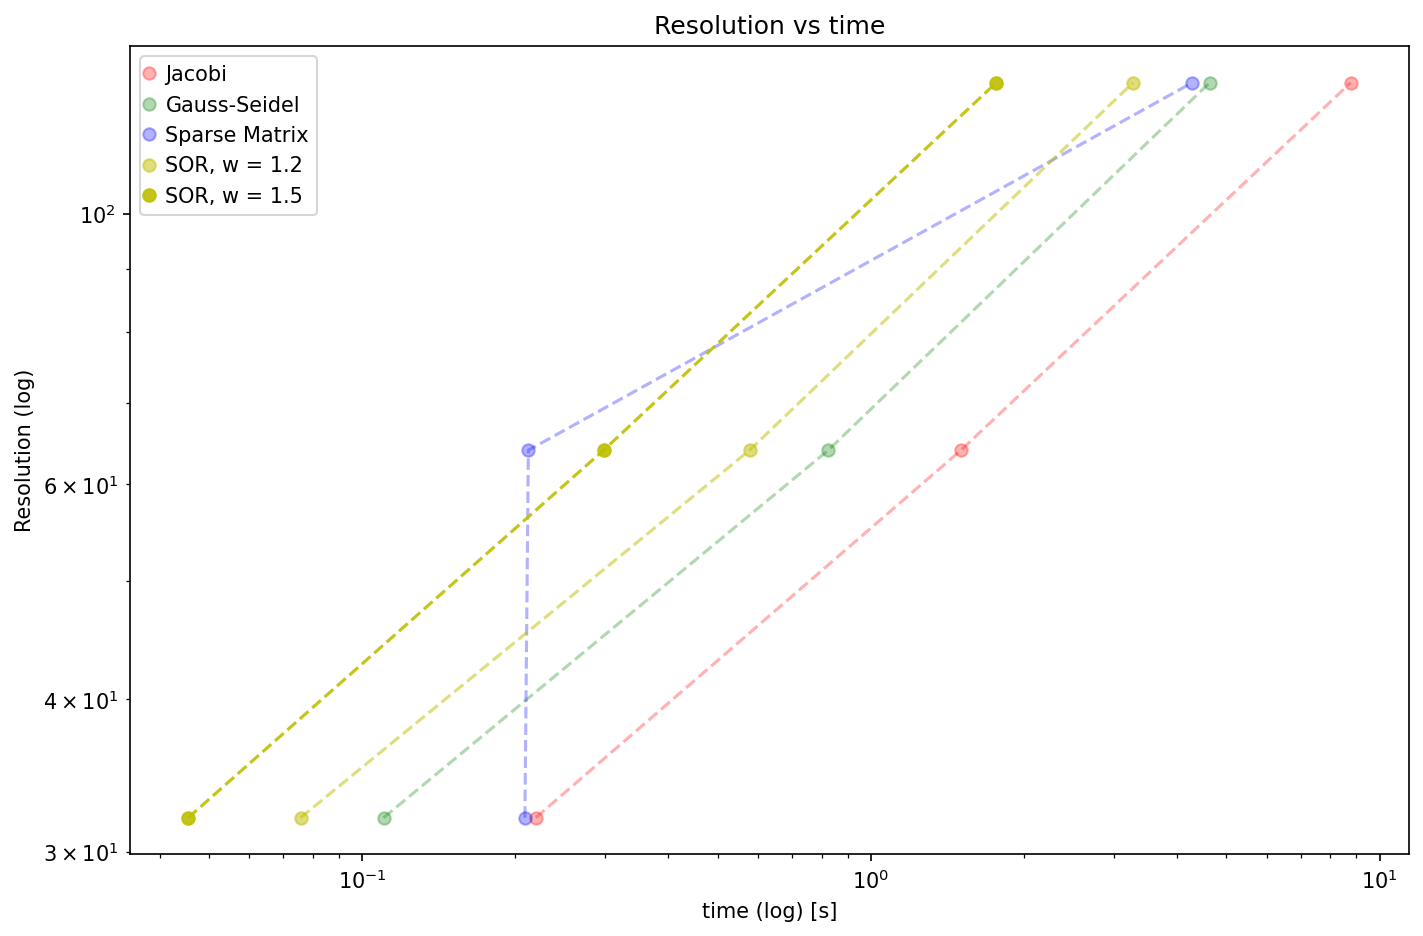
\includegraphics[width = 0.45\textwidth]{./RK4/4.png}  
    %     \includegraphics[width = 0.45\textwidth]{./RK4/6.png}
    %     \includegraphics[width = 0.45\textwidth]{./RK4/8.png}
    %     \includegraphics[width = 0.45\textwidth]{./RK4/10.png} 
    %     \caption{This the normal cloud with RK4, from $t=0$ to $t=10$ and $dt=0.01$.}
    %     \label{RK4_cloud}
    % \end{figure}

    \section{Programming Assignments}
    \subsection{(2) Leapfrog method}


    \subsection{(3) Energy comparison}


\section{Codes}
    All the codes are transferred from jupyterlab or python codes; hence, if you want to re-run them, please see the source code in the attached files or my GitHub repository: \newline
    {\centerline{\ttfamily <https://github.com/gary20000915/Comphyslab-HW4.git>}}

    \subsection{{\ttfamily\ particles.py}}
        \begin{lstlisting}[language={Python}]
        
        \end{lstlisting}

\end{document}